% Preamble
\documentclass[11pt]{article}

% Packages
\usepackage{amsmath}
\usepackage[a4paper, margin=0.5in]{geometry}
\usepackage{graphicx} % daj an 1in jak chcesz normalniejszy margines, ale kod mi się w linii nie mieści :P

\title{Zadanie 1. Heurystyki konstrukcyjne}
\author{Oskar Kiliańczyk 151863 \& Wojciech Kot 151876}
\date{}

% Document
\begin{document}

\maketitle
\newpage

\section{Opis zadania}\label{sec:opis-zadania}

Podczas zajęć rozważamy zmodyfikowany problem komiwojażera.
Początkowo, obliczamy macierz odległości pomiędzy danymi miastami.
Obliczona macierz odległości między wierzchołkami grafu będzie podstawą dla każdego algorytmu,
a celem jest wyznaczenie dwóch rozłącznych zamkniętych ścieżek (cykli), z których każda zawiera 50\% wierzchołków.
Jeśli liczba wierzchołków jest nieparzysta, jedna ścieżka zawiera jeden wierzchołek więcej.
Kryterium optymalizacji jest minimalizacja łącznej długości obu cykli.

Rozważane instancje problemu pochodzą z biblioteki TSPLib, a są to kroa200 oraz krob200.
Są to instancje dwuwymiarowe euklidesowe, w których każdemu wierzchołkowi przypisane są współrzędne na płaszczyźnie.
Odległość między wierzchołkami liczona jest jako odległość euklidesowa, zaokrąglana do najbliższej liczby całkowitej.
W implementacji algorytmów wykorzystywana będzie wyłącznie macierz odległości, co zapewnia możliwość zastosowania kodu do innych instancji problemu.

\section{Zaimplementowane algorytmy}\label{sec:zaimplementowane-algorytmy}

\subsection{Algorytm zachłanny - metoda najbliższego sąsiada}\label{subsec:algorytm-zachanny---metoda-najblizszego-sasiada}

Algorytm ten wykorzystuje funkcję znajdującą najbliższego sąsiada dla danego wierzchołka (miasta)
Działa ona w następujący sposób: \\
dla każdego miasta, sprawdza czy zostało już odwiedzone \\
jeśli nie, to sprawdza czy dystans jest mniejszy od dystansu z danego miasta do obecnie zapamiętanego jako najbliższe \\
jeśli jest bliższe niż obecnie pamiętane jako najbliższe, zapamiętuje je jako najbliższe \\
jeśli nie ma żadnego miasta obecnie pamiętanego jako najbliższe, przypisuje to miasto \\

Główny algorytm natomiast, wygląda następująco: \\

\begin{verbatim}
    Przydziela wierzchołki startowe do cykli pierwszego i drugiego
    Tworzy tablicę indeksów miast, zaznaczając wszystkie poza startowymi jako nieodwiedzone
    dopóki istnieją jakieś nieodwiedzone miasta, powtarza następujące 4 kroki:
        Znajduje najbliższego nieodwiedzonego sąsiada do ostatniego wierzchołka cyklu 1.
        dodaje go do cyklu1 oraz zapisuje w tablicy jako odwiedzony
        Znajduje najbliższego nieodwiedzonego sąsiada do ostatniego wierzchołka cyklu 2.
        dodaje go do cyklu2 oraz zapisuje w tablicy jako odwiedzony
    Kiedy już nie ma żadnych nieodwiedzonych miast, dopisuje na koniec cykli ich wierzchołki startowe
    Zwraca oba cykle jako znalezione ścieżki

\end{verbatim}

\subsection{Algorytm zachłanny - metoda rozbudowy cyklu}\label{subsec:algorytm-zachanny---metoda-rozbudowy-cyklu}

Algorytm ten korzysta z funkcji znajdywania najlepszego wstawienia, a działa ona w następujący sposób:

\begin{verbatim}
    Przyjmuje jako argumenty obecny cykl, macierz dystansów, oraz tablicę indeksów odwiedzonych miast
    Tworzy listę możliwości (nieodwiedzonych wierzchołków)
    ustawia najtańszy koszt na maksymalnie dużą wartość
    dla każdej możliwości z listy możliwości:
        dla każdego możliwego wstawienia w cykl:
             - oblicza wzrost dystansu, jaki spowoduje wstawienie (a więc przy wstawianiu między a i b wierzchołka c, oblicza dystans ac + bc - ab)
             - zapisuje najmniejszy znaleziony wzrost dystansu oraz miejsce jego wstawienia
        jeśli koszt wstawienia obecnie znalezionego wierzchołka jest mniejszy niż obecnie pamiętany najtańszy koszt wstawienia, zapisuje ten koszt jako obecnie najtańszy, oraz wierzchołek i miejsce jego wstawienia
    Po przejrzeniu wszystkich możliwości zwraca parę <wierzchołek, miejsce wstawienia>

\end{verbatim}

\begin{verbatim}
    Dwukrotnie przydziela wierzchołki startowe do cykli pierwszego i drugiego jako początek i koniec cyklu)
    Tworzy tablicę indeksów miast, zaznaczając wszystkie poza startowymi jako nieodwiedzone
    dopóki istnieją jakieś nieodwiedzone miasta, powtarza następujące 7 kroków:
        Znajduje najtańsze wstawienie, czyli parę <wierzchołek, miejsce w cyklu> dla cyklu 1
        Wstawia w odpowiednie miejsce cyklu 1 znaleziony wierzchołek
        Zapisuje wierzchołek jako już odwiedzony
        Znajduje najtańsze wstawienie dla cyklu 2
        Jeśli ono nie istnieje (np. bo ostatni wierzchołek został już wstawiony) to kończy pętlę
        Wstawia w odpowiednie miejsce cyklu 2 znaleziony wierzchołek
        Zapisuje wierzchołek jako już odwiedzony
    Kiedy już nie ma żadnych nieodwiedzonych miast zwraca oba cykle jako znalezione ścieżki

\end{verbatim}

\subsection{Algorytm z żalem - metoda rozbudowy cyklu}\label{subsec:algorytm-z-zalem---metoda-rozbudowy-cyklu}

\begin{verbatim}
    kodkodkod
\end{verbatim}

\subsection{Algorytm z żalem - metoda rozbudowy cyklu z żalem ważonym}\label{subsec:algorytm-z-zalem---metoda-rozbudowy-cyklu-z-zalem-wazonym}

\begin{verbatim}
    kodkodkod
\end{verbatim}

\subsection{Własny jakiś dziki algorytm, jak nam się będzie chciało, bo imo bym zrobił coś}

\begin{verbatim}
    kodkodkod
\end{verbatim}


\section{Wyniki eksperymentu obliczeniowego}\label{sec:wyniki-eksperymenty-obliczeniowego}

\subsection{Algorytm zachłanny - metoda najbliższego sąsiada}\label{subsec:algorytm-zachanny---metoda-najblizszego-sasiada2}

Graficzną reprezentację wyników dla algorytmu zachłannego metodą najbliższego sąsiada przestawiono na~\ref{fig:Greedy-nearest-kroA, fig:Greedy-nearest-kroB}
\begin{figure}[H]
    \centering
    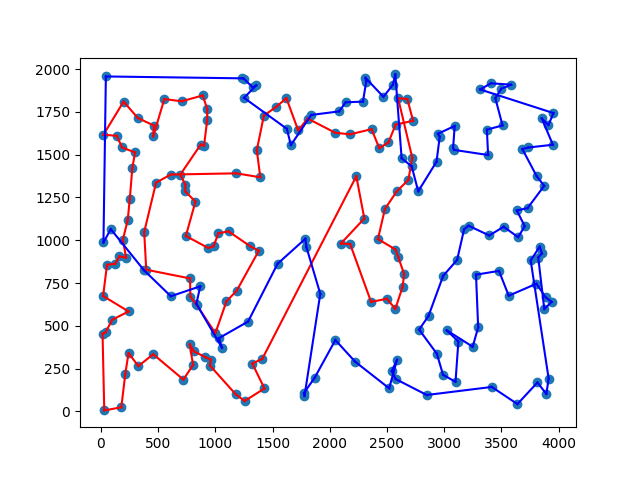
\includegraphics{best_paths/greedy_nearest_neighbor_kroA200.tsp}
    \caption{Instancja kroA200}
    \label{fig:Greedy-nearest-kroA}
\end{figure}
\begin{figure}[H]
    \centering
    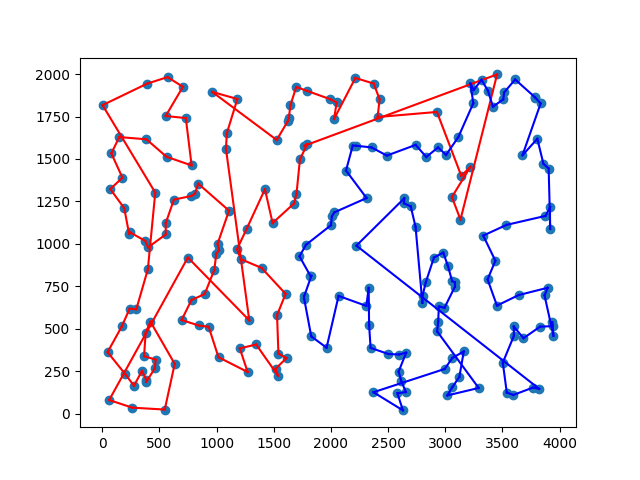
\includegraphics{best_paths/greedy_nearest_neighbor_kroB200.tsp}
    \caption{Instancja kroB200}
    \label{fig:Greedy-nearest-kroB}
\end{figure}


\subsection{Algorytm zachłanny - metoda rozbudowy cyklu}\label{subsec:algorytm-zachanny---metoda-rozbudowy-cyklu2}

Graficzną reprezentację wyników dla algorytmu zachłannego metodą rozbudowy cyklu przestawiono na~\ref{fig:Greedy-cycle-kroA, fig:Greedy-cycle-kroB}
\begin{figure}[H]
    \centering
    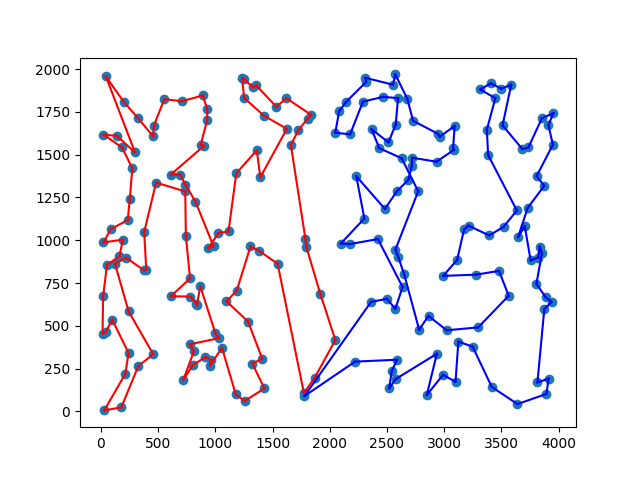
\includegraphics{best_paths/greedy_cheapest_insertion_kroA200.tsp}
    \caption{Instancja kroA200}
    \label{fig:Greedy-cycle-kroA}
\end{figure}
\begin{figure}[H]
    \centering
    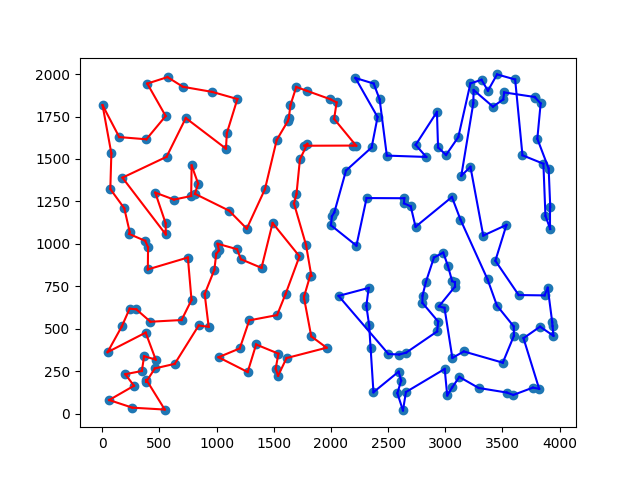
\includegraphics{best_paths/greedy_cheapest_insertion_kroB200.tsp}
    \caption{Instancja kroB200}
    \label{fig:Greedy-cycle-kroB}
\end{figure}

\section{Wnioski}\label{sec:wnioski}

Żal nie działa, chociaż byśmy chcieli, ale żal rozwiązuje zwykły TSP.
Może w połączeniu z algorytmem klastrującym, jakimś k-means zadziałałby lepiej, ale strasznie krzywdzące dla niego jest też to że ścieżki MUSZĄ być równej długości

\section{Link do repo}\label{sec:link-do-repo}

\end{document}
